\documentclass{../source/Experiment}

\major{信息工程}
\name{姚桂涛}
\title{有限长序列、频谱、DFT的性质}
\stuid{3190105597}
\college{信息与电子工程学院}
\date{\today}
\lab{——}
\course{数字信号处理}
\instructor{徐元欣}
\grades{}
\expname{有限长序列、频谱、DFT的性质}
\exptype{演示}
\partner{——}
\begin{document}
    \makeheader
    \section{实验目的和要求}
    设计通过演示实验,建立对典型信号及其频谱的直观认识,理解DFT的物理意义、主要性质。

    \section{实验内容和步骤}
    2-1 用MATLAB,计算得到五种共9个序列:
    \begin{figure}[H]
        \centering
        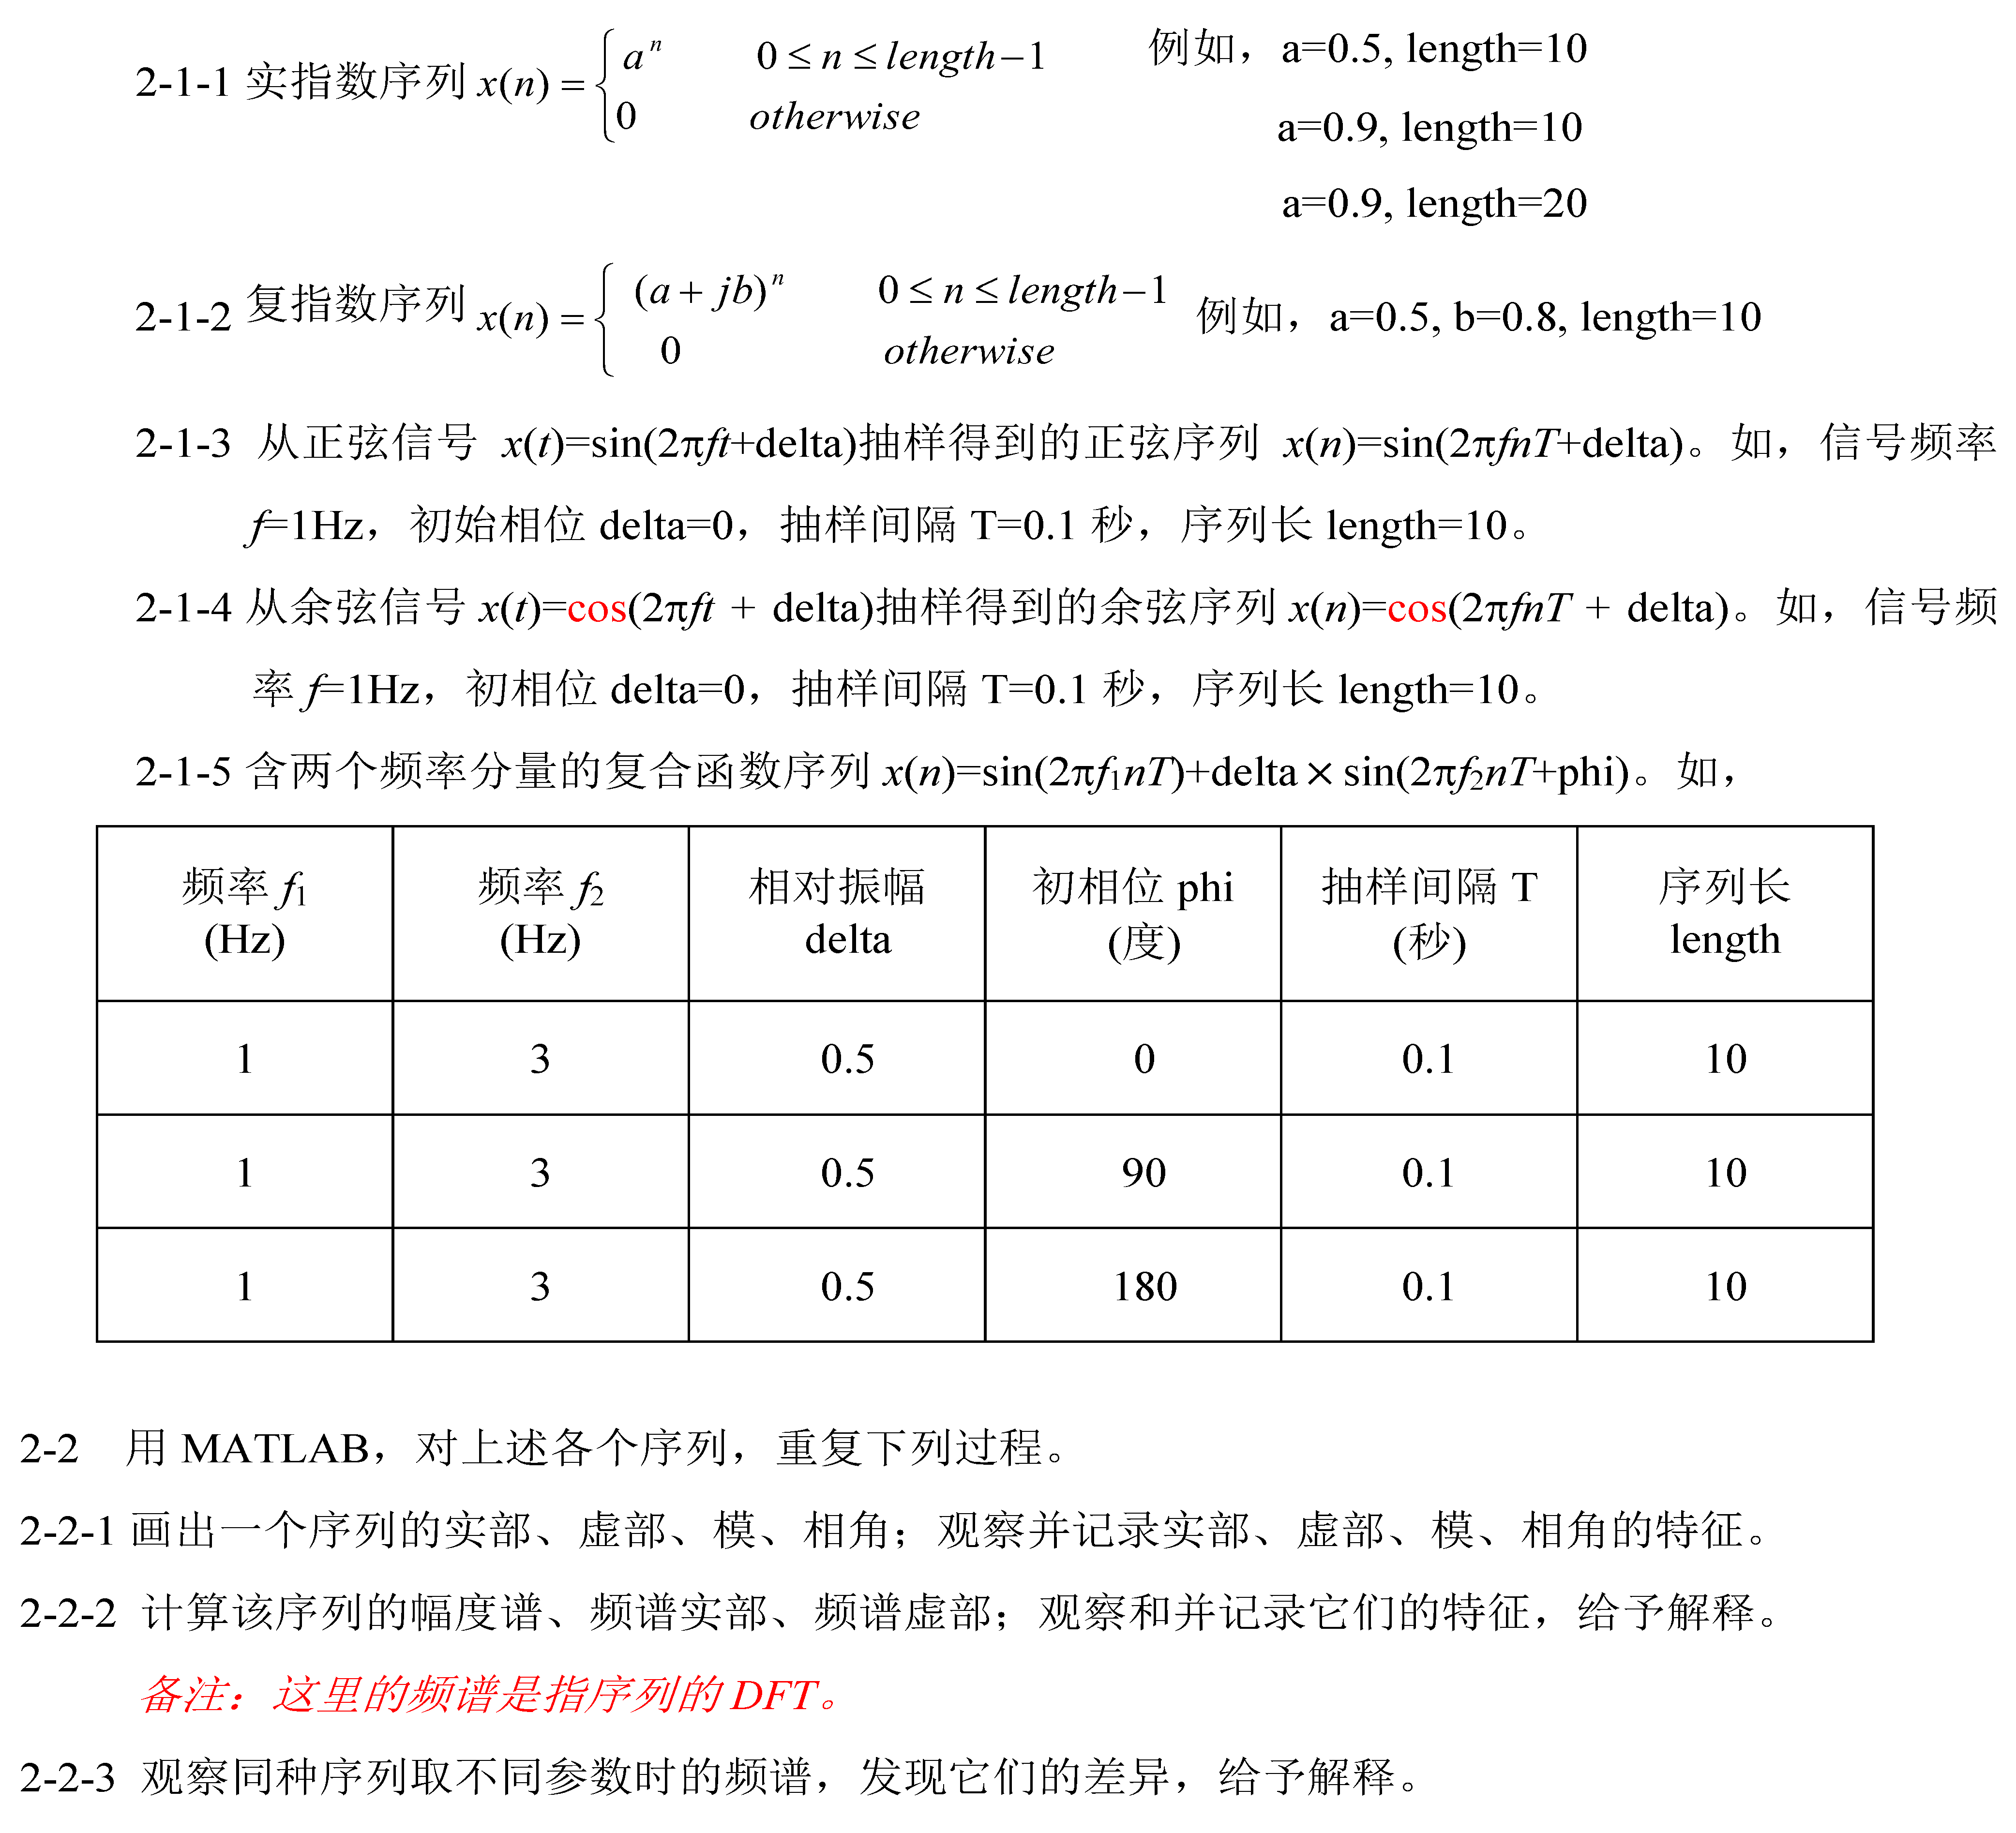
\includegraphics[width = 0.90\textwidth]{pic/2.png}
    \end{figure}
    \newpage

    \section{主要仪器设备}
    
    MATLAB编程。

    \section{操作方法和实验步骤}

    (参见“二、实验内容和步骤”)

    \section{实验数据记录和处理}
    
        MATLAB程序清单
        \subsection{各序列主函数}
            \subsubsection{2-1-1:$x(n)= \begin{cases}a^{n} & 0 \leq n \leq \text { length }-1 \\ 0 & \text { otherwise }\end{cases}$}
            \lstinputlisting[
                language       =   Matlab,
                title     =   {2-1-1a}
            ]{src/sol2_1_1a.m}
            \lstinputlisting[
                language       =   Matlab,
                title     =   {2-1-1b}
            ]{src/sol2_1_1b.m}
            \lstinputlisting[
                language       =   Matlab,
                title     =   {2-1-1c}
            ]{src/sol2_1_1c.m}
            \subsubsection{2-1-2:$x(n)=\left\{\begin{array}{cl}(a+j b)^{n} & 0 \leq n \leq \text { length }-1 \\ 0 & \text { otherwise }\end{array}\right.$}
            \lstinputlisting[
                language       =   Matlab,
                title     =   {2-1-2}
            ]{src/sol2_1_2.m}

            \subsubsection{从正弦信号$x(t)=sin(2\pi ft+delta)$抽样得到的正弦序列$x(n)=sin(2\pi fnT+delta)$。}
            \lstinputlisting[
                language       =   Matlab,
                title     =   {2-1-3}
            ]{src/sol2_1_3.m}

            \subsubsection{从余弦信号$x(t)=cos(2\pi ft+delta)$抽样得到的余弦序列$x(n)=cos(2\pi fnT+delta)$。}
            \lstinputlisting[
                language       =   Matlab,
                title     =   {2-1-4}
            ]{src/sol2_1_4.m}
            
            \subsubsection{含两个频率分量的复合函数序列$x(n)=sin(2\pi f_1 n T)+delta \times sin(2\pi f_2 nT+phi)$。}

            \begin{table}[H]
                \centering
                \begin{tabular}{|c|c|c|c|c|c|c|}
                \hline
                  & \begin{tabular}[c]{@{}c@{}}频率$f_1$\\ (Hz)\end{tabular} & \begin{tabular}[c]{@{}c@{}}频率$f_2$\\ (Hz)\end{tabular} & \begin{tabular}[c]{@{}c@{}}相对振幅\\ $delta$\end{tabular} & \begin{tabular}[c]{@{}c@{}}初相位$phi$\\ (度)\end{tabular} & \begin{tabular}[c]{@{}c@{}}抽样间隔$T$\\ (秒)\end{tabular} & \begin{tabular}[c]{@{}c@{}}序列长\\ $length$\end{tabular} \\ \hline
                a & 1                                                      & 3                                                      & 0.5                                                    & 0                                                      & 0.1                                                   & 10                                                     \\ \hline
                b & 1                                                      & 3                                                      & 0.5                                                    & 90                                                     & 0.1                                                   & 10                                                     \\ \hline
                c & 1                                                      & 3                                                      & 0.5                                                    & 180                                                    & 0.1                                                   & 10                                                     \\ \hline
                \end{tabular}
            \end{table}

            \lstinputlisting[
                language       =   Matlab,
                title     =   {2-1-5a}
            ]{src/sol2_1_5a.m}
            \lstinputlisting[
                language       =   Matlab,
                title     =   {2-1-5b}
            ]{src/sol2_1_5b.m}
            \lstinputlisting[
                language       =   Matlab,
                title     =   {2-1-5c}
            ]{src/sol2_1_5c.m}

            \subsection{DFT函数:求出序列的DFT}
            \lstinputlisting[
                language       =   Matlab,
                title     =   {DFT函数}
            ]{src/myDFT.m}

            \subsection{绘图函数:绘制序列的实部、虚部、模、相角图以及幅度谱、频谱实部、频谱虚部图}
            \lstinputlisting[
                language       =   Matlab,
                title     =   {绘图函数}
            ]{src/myPlot.m}

    \section{实验结果与分析}
        \subsection{序列各图像特征与解释}

            \subsubsection{2-1-1:$x(n)= \begin{cases}a^{n} & 0 \leq n \leq \text { length }-1 \\ 0 & \text { otherwise }\end{cases}$}

            \begin{figure}[H]
                \centering
                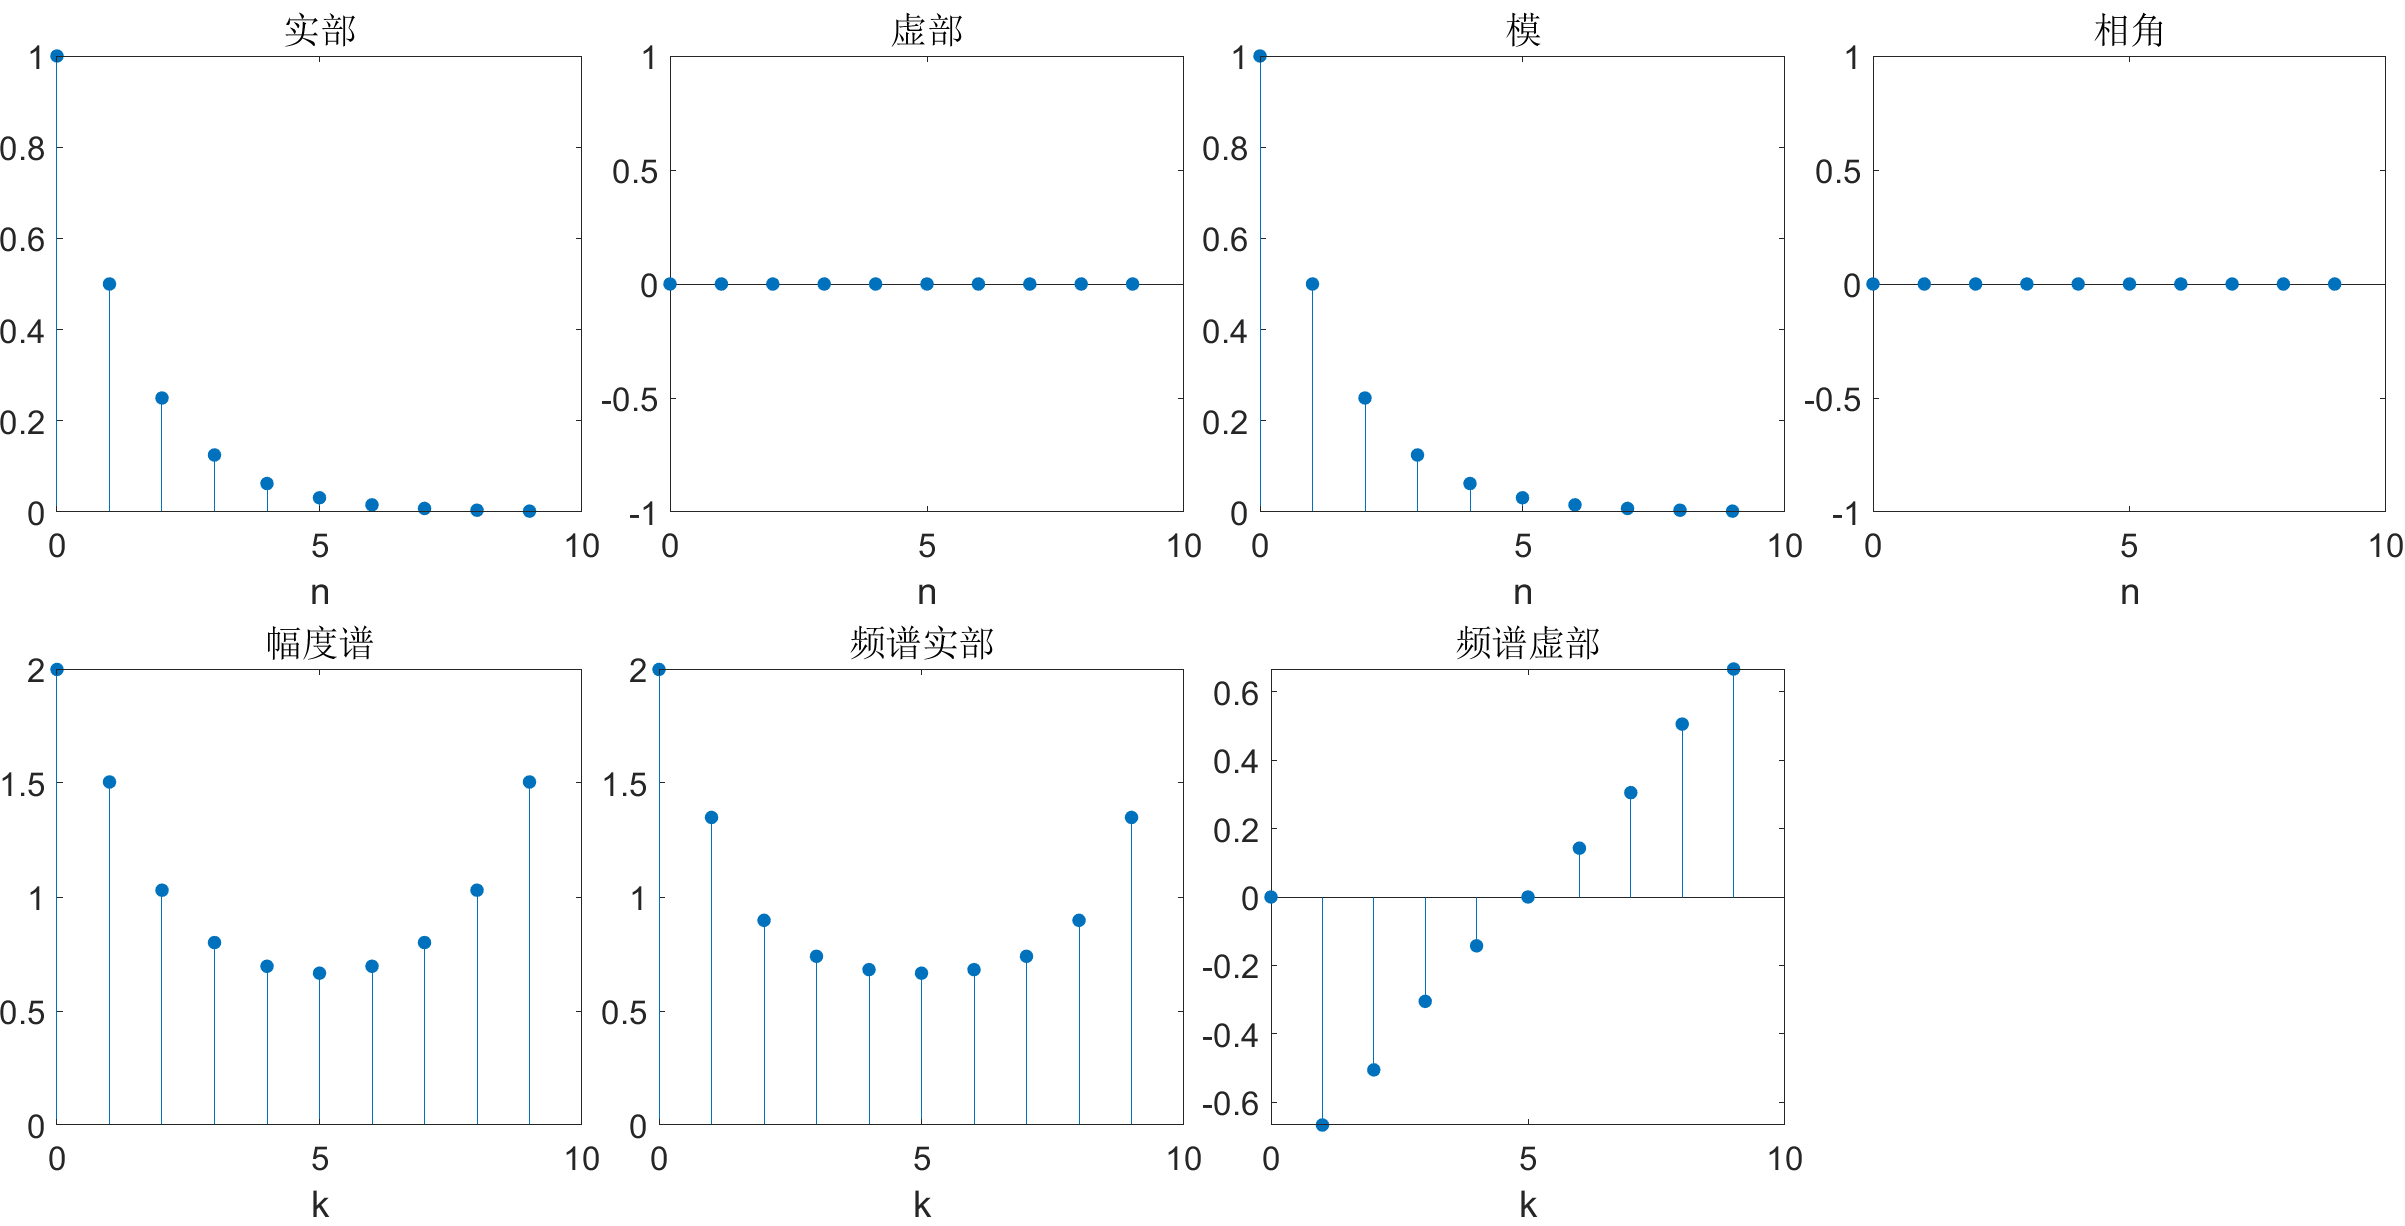
\includegraphics[width = \textwidth]{src/2_1_1a}
                \caption{a = 0.5, length = 10}
            \end{figure}
            
            \begin{figure}[H]
                \centering
                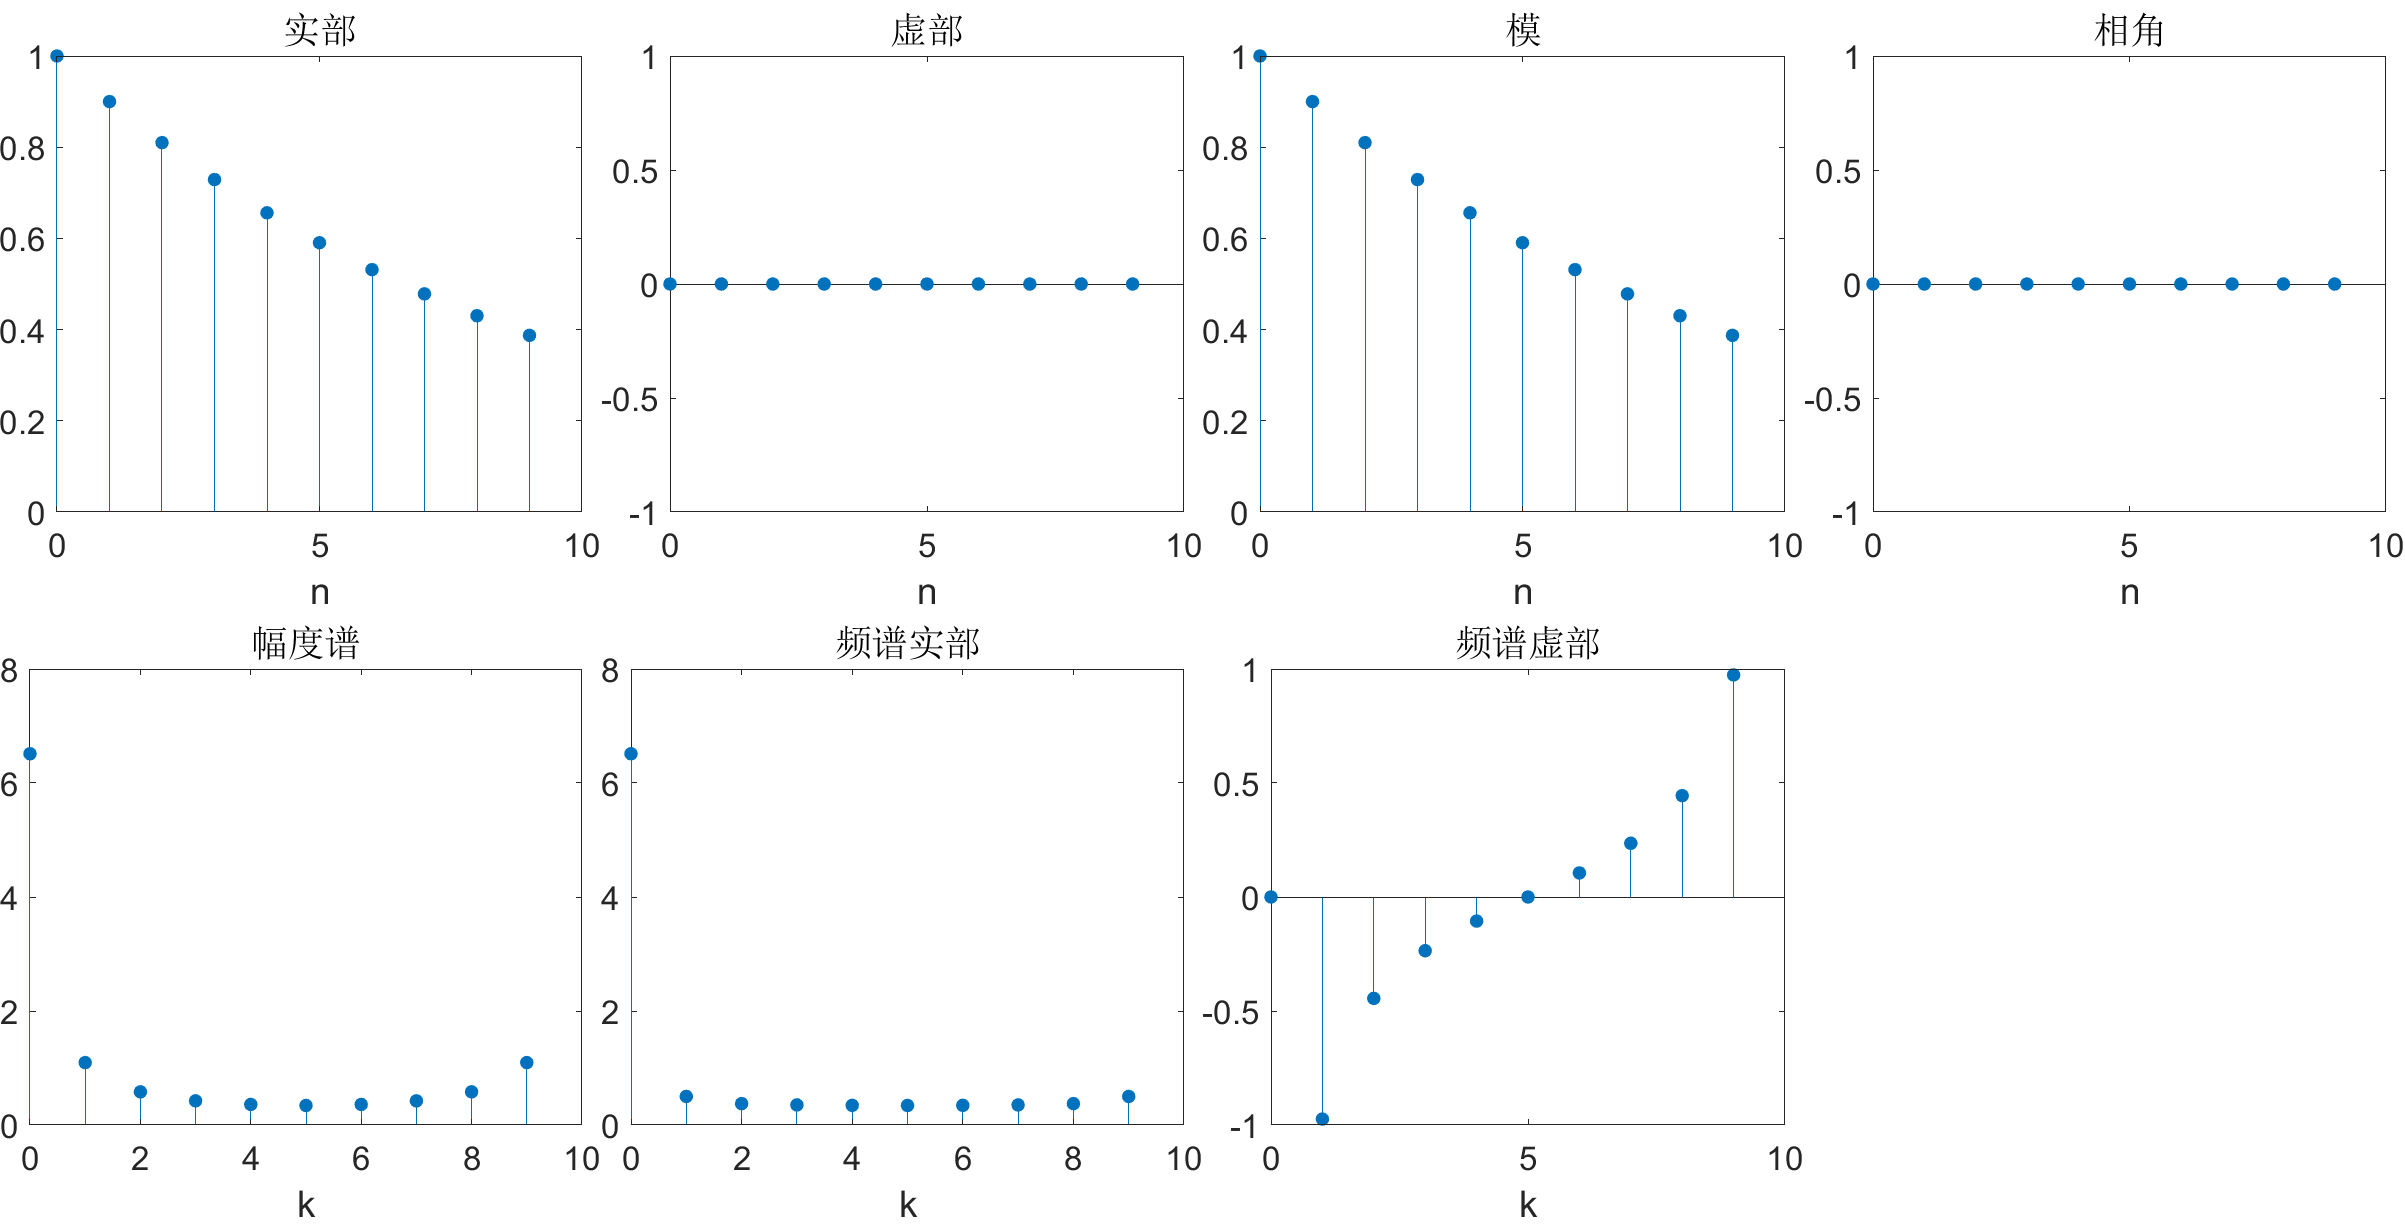
\includegraphics[width = \textwidth]{src/2_1_1b}
                \caption{a = 0.9, length = 10}
            \end{figure}

            \begin{figure}[H]
                \centering
                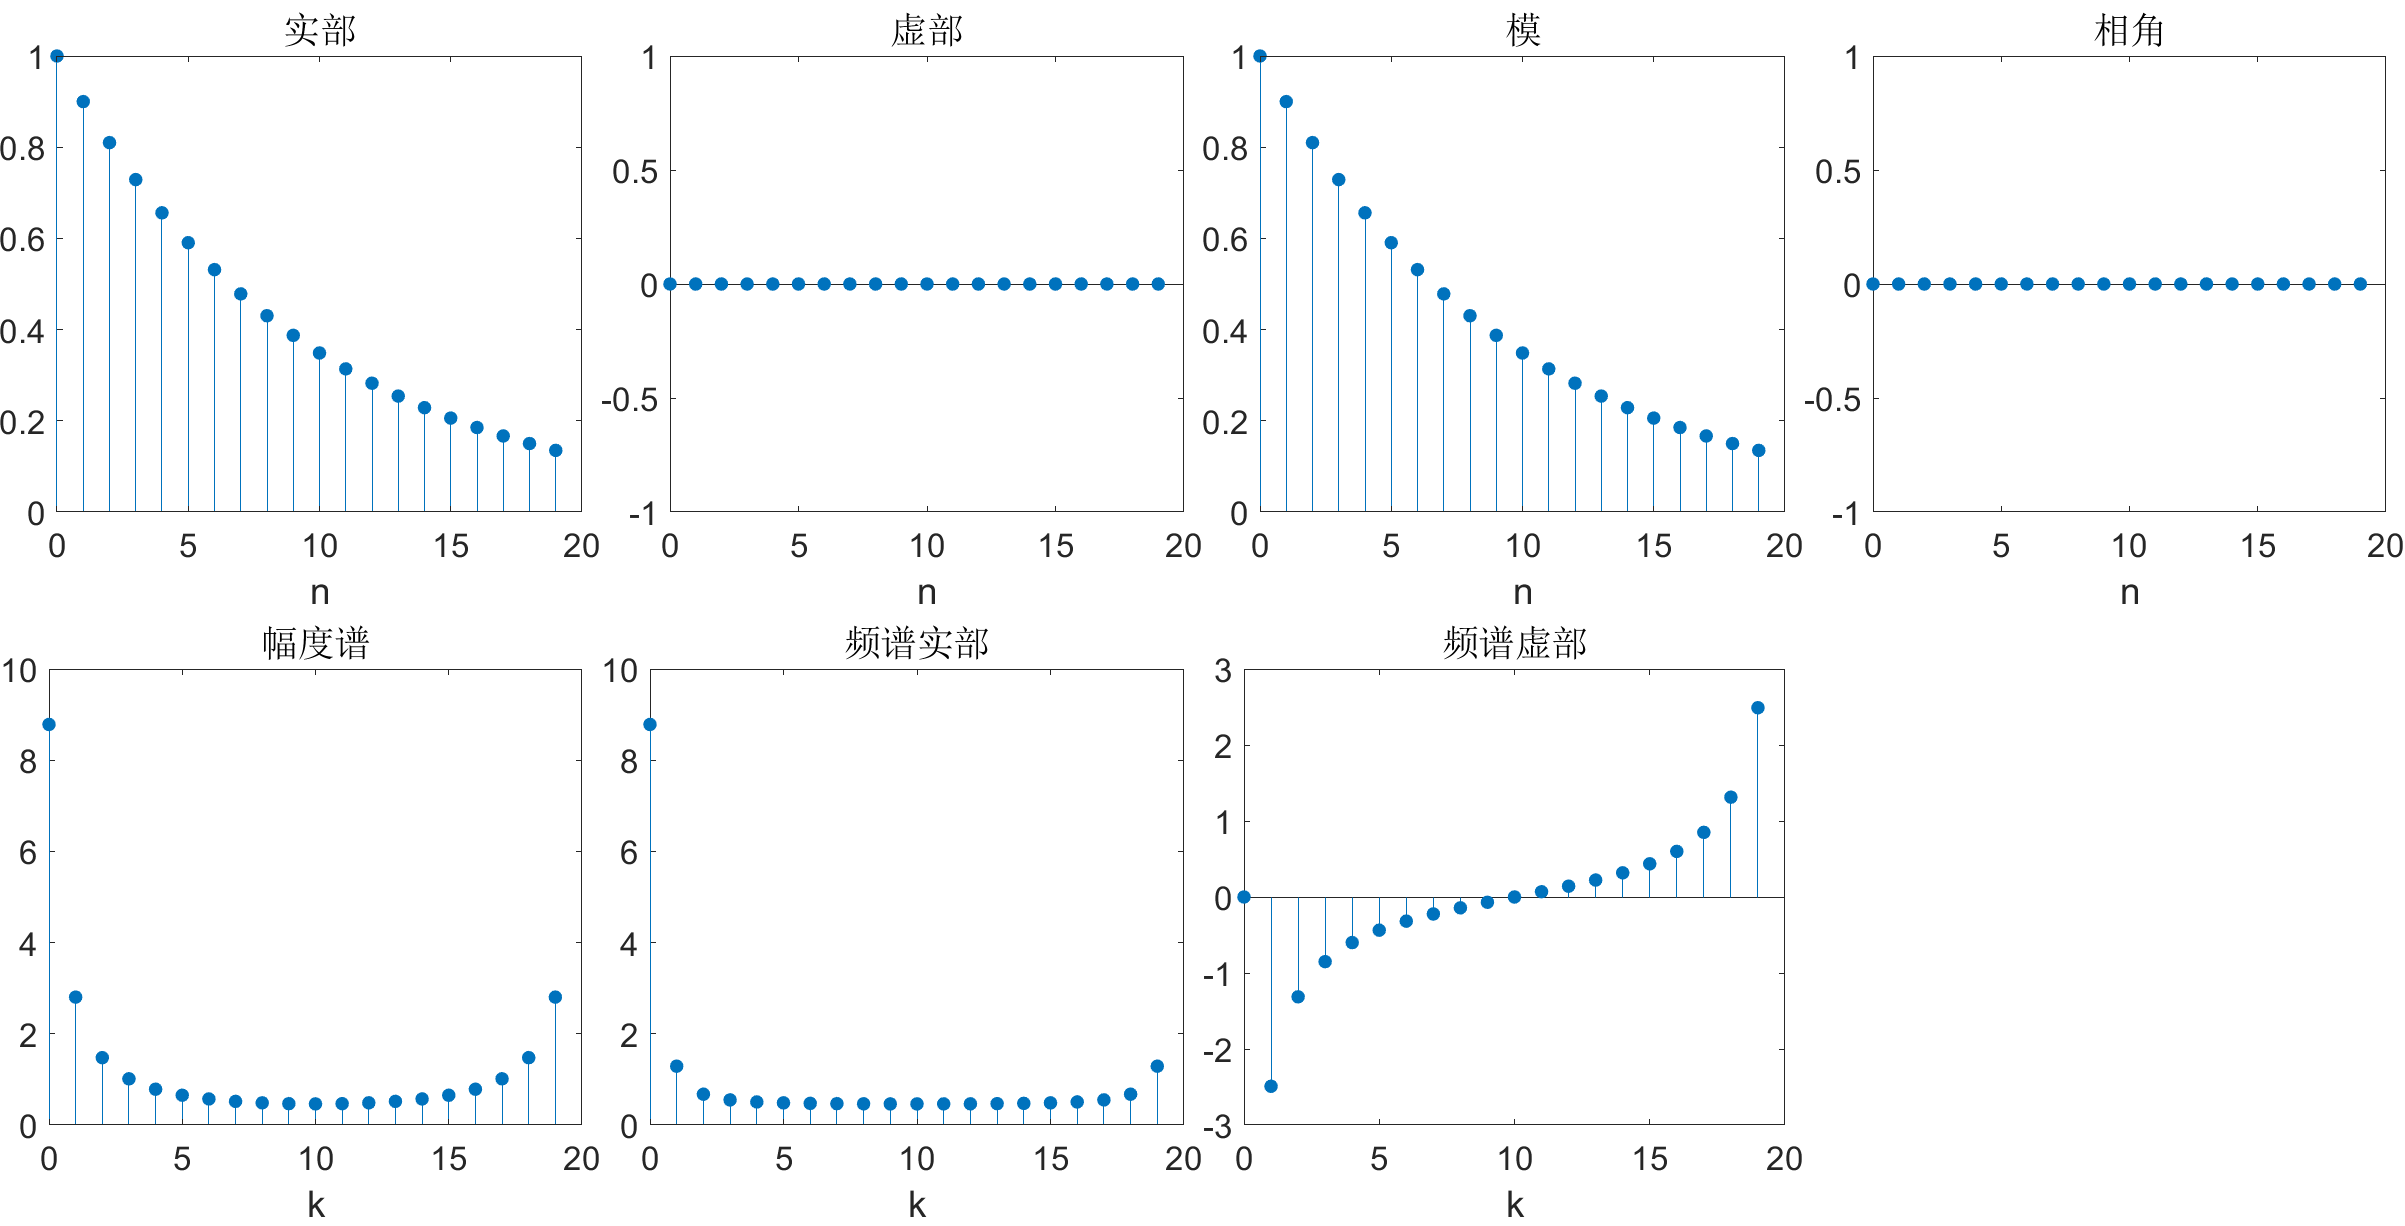
\includegraphics[width = \textwidth]{src/2_1_1c}
                \caption{a = 0.9, length = 20}
            \end{figure}
            
            由时域图像可知,由于是实指数序列,其序列和相位为零,并且a增大时,模减小越慢。
            由频域图像可知,其实部具有偶对称性,虚部具有奇对称性。这符合了我们所学的实数序列的性质。
            且分析不同参数图像可知,length越大,频谱越能反映出真实图像,其原因采样率提高了。

            \subsubsection{2-1-2:$x(n)=\left\{\begin{array}{cl}(a+j b)^{n} & 0 \leq n \leq \text { length }-1 \\ 0 & \text { otherwise }\end{array}\right.$}

            \begin{figure}[H]
                \centering
                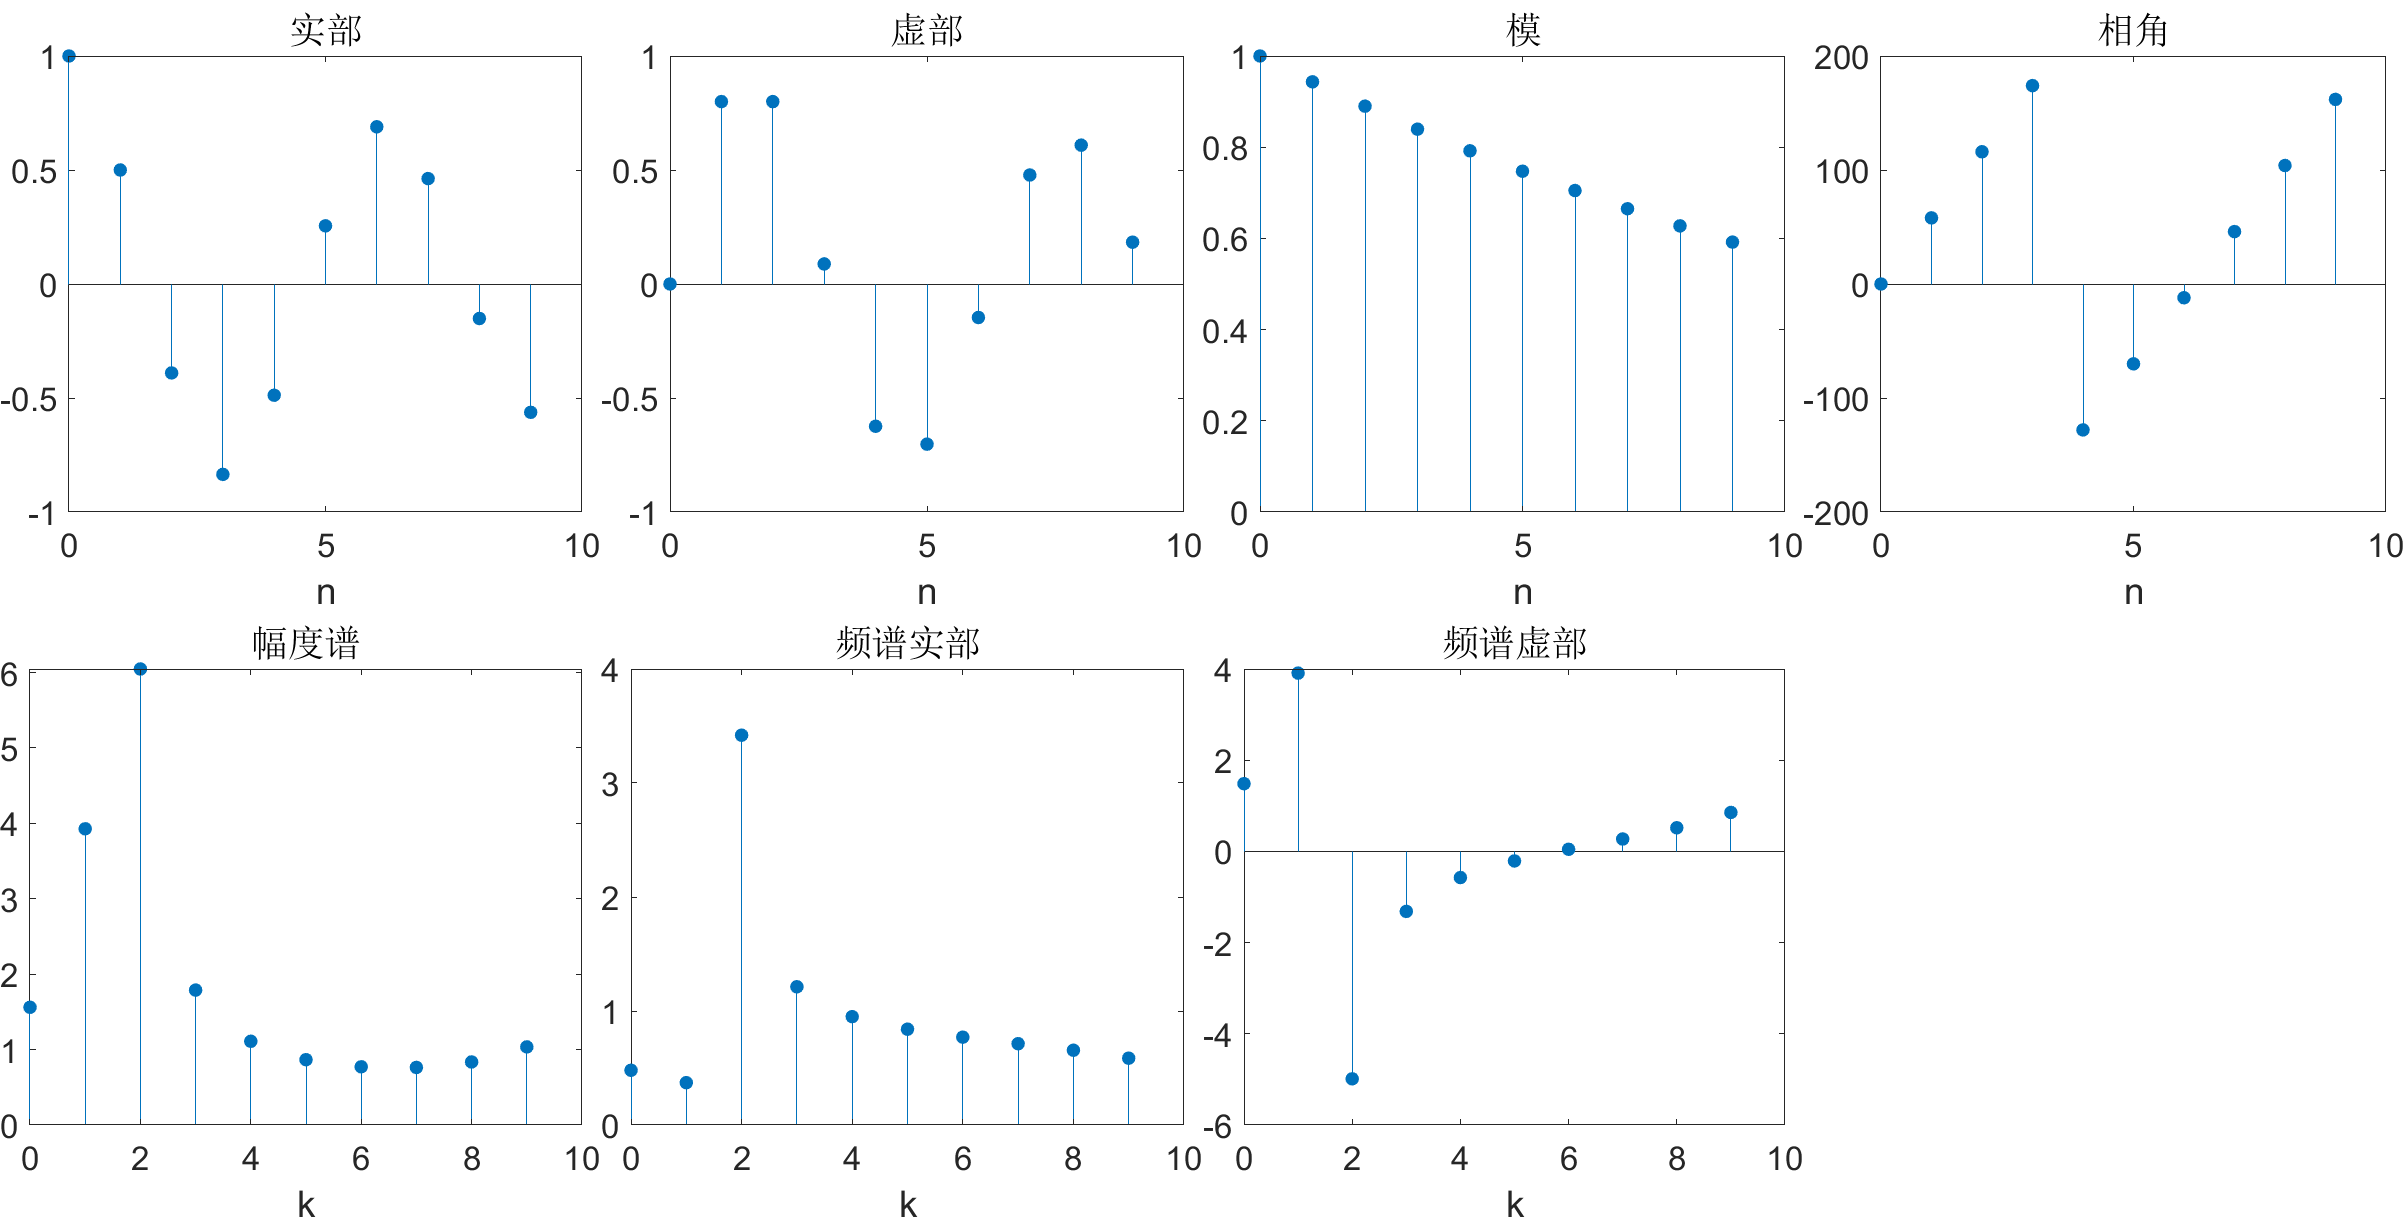
\includegraphics[width = \textwidth]{src/2_1_2}
                \caption{复指数序列}
            \end{figure}

            由时域图像可知,由于是复指数序列,其实部和虚部呈现出正弦函数的特性。
            分析频域图像,并未发现明显特点。

            \subsubsection{从正弦信号$x(t)=sin(2\pi ft+delta)$抽样得到的正弦序列$x(n)=sin(2\pi fnT+delta)$。}

            \begin{figure}[H]
                \centering
                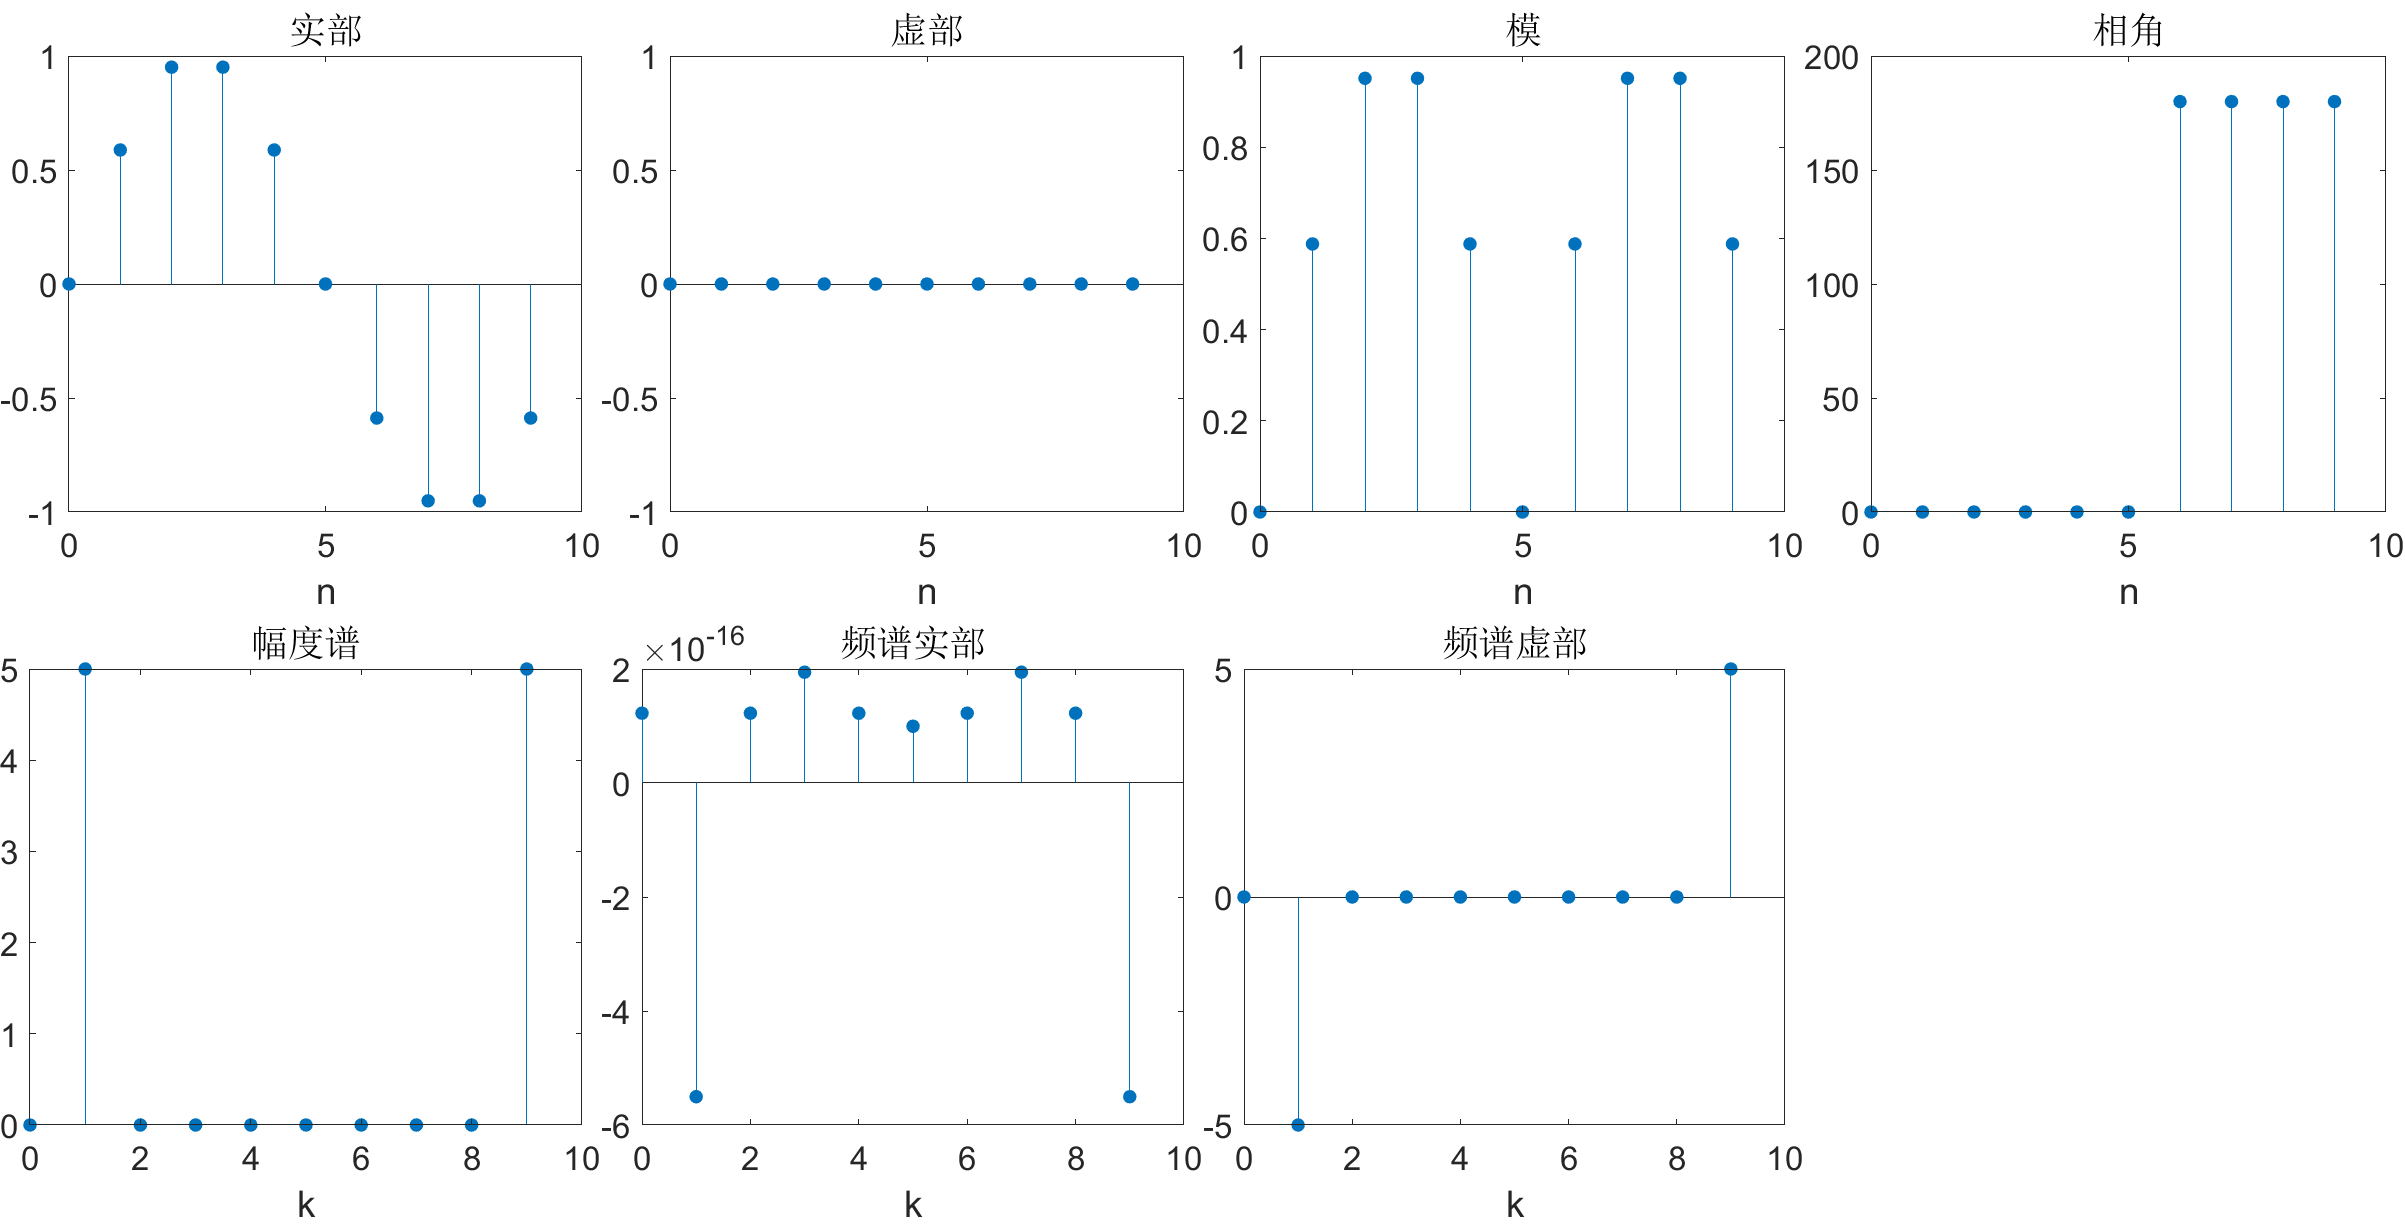
\includegraphics[width = \textwidth]{src/2_1_3.png}
                \caption{正弦函数抽样序列}
            \end{figure}

            由时域图可知,此序列为奇对称序列。模为偶对称,且其相位在x(n)小于零时为0,在大于零时为180\degree
            由频域图可知,由于此序列为奇对称序列,所以其频谱实部趋于零,虚部奇对称。

            \subsubsection{从余弦信号$x(t)=cos(2\pi ft+delta)$抽样得到的余弦序列$x(n)=cos(2\pi fnT+delta)$。}

            \begin{figure}[H]
                \centering
                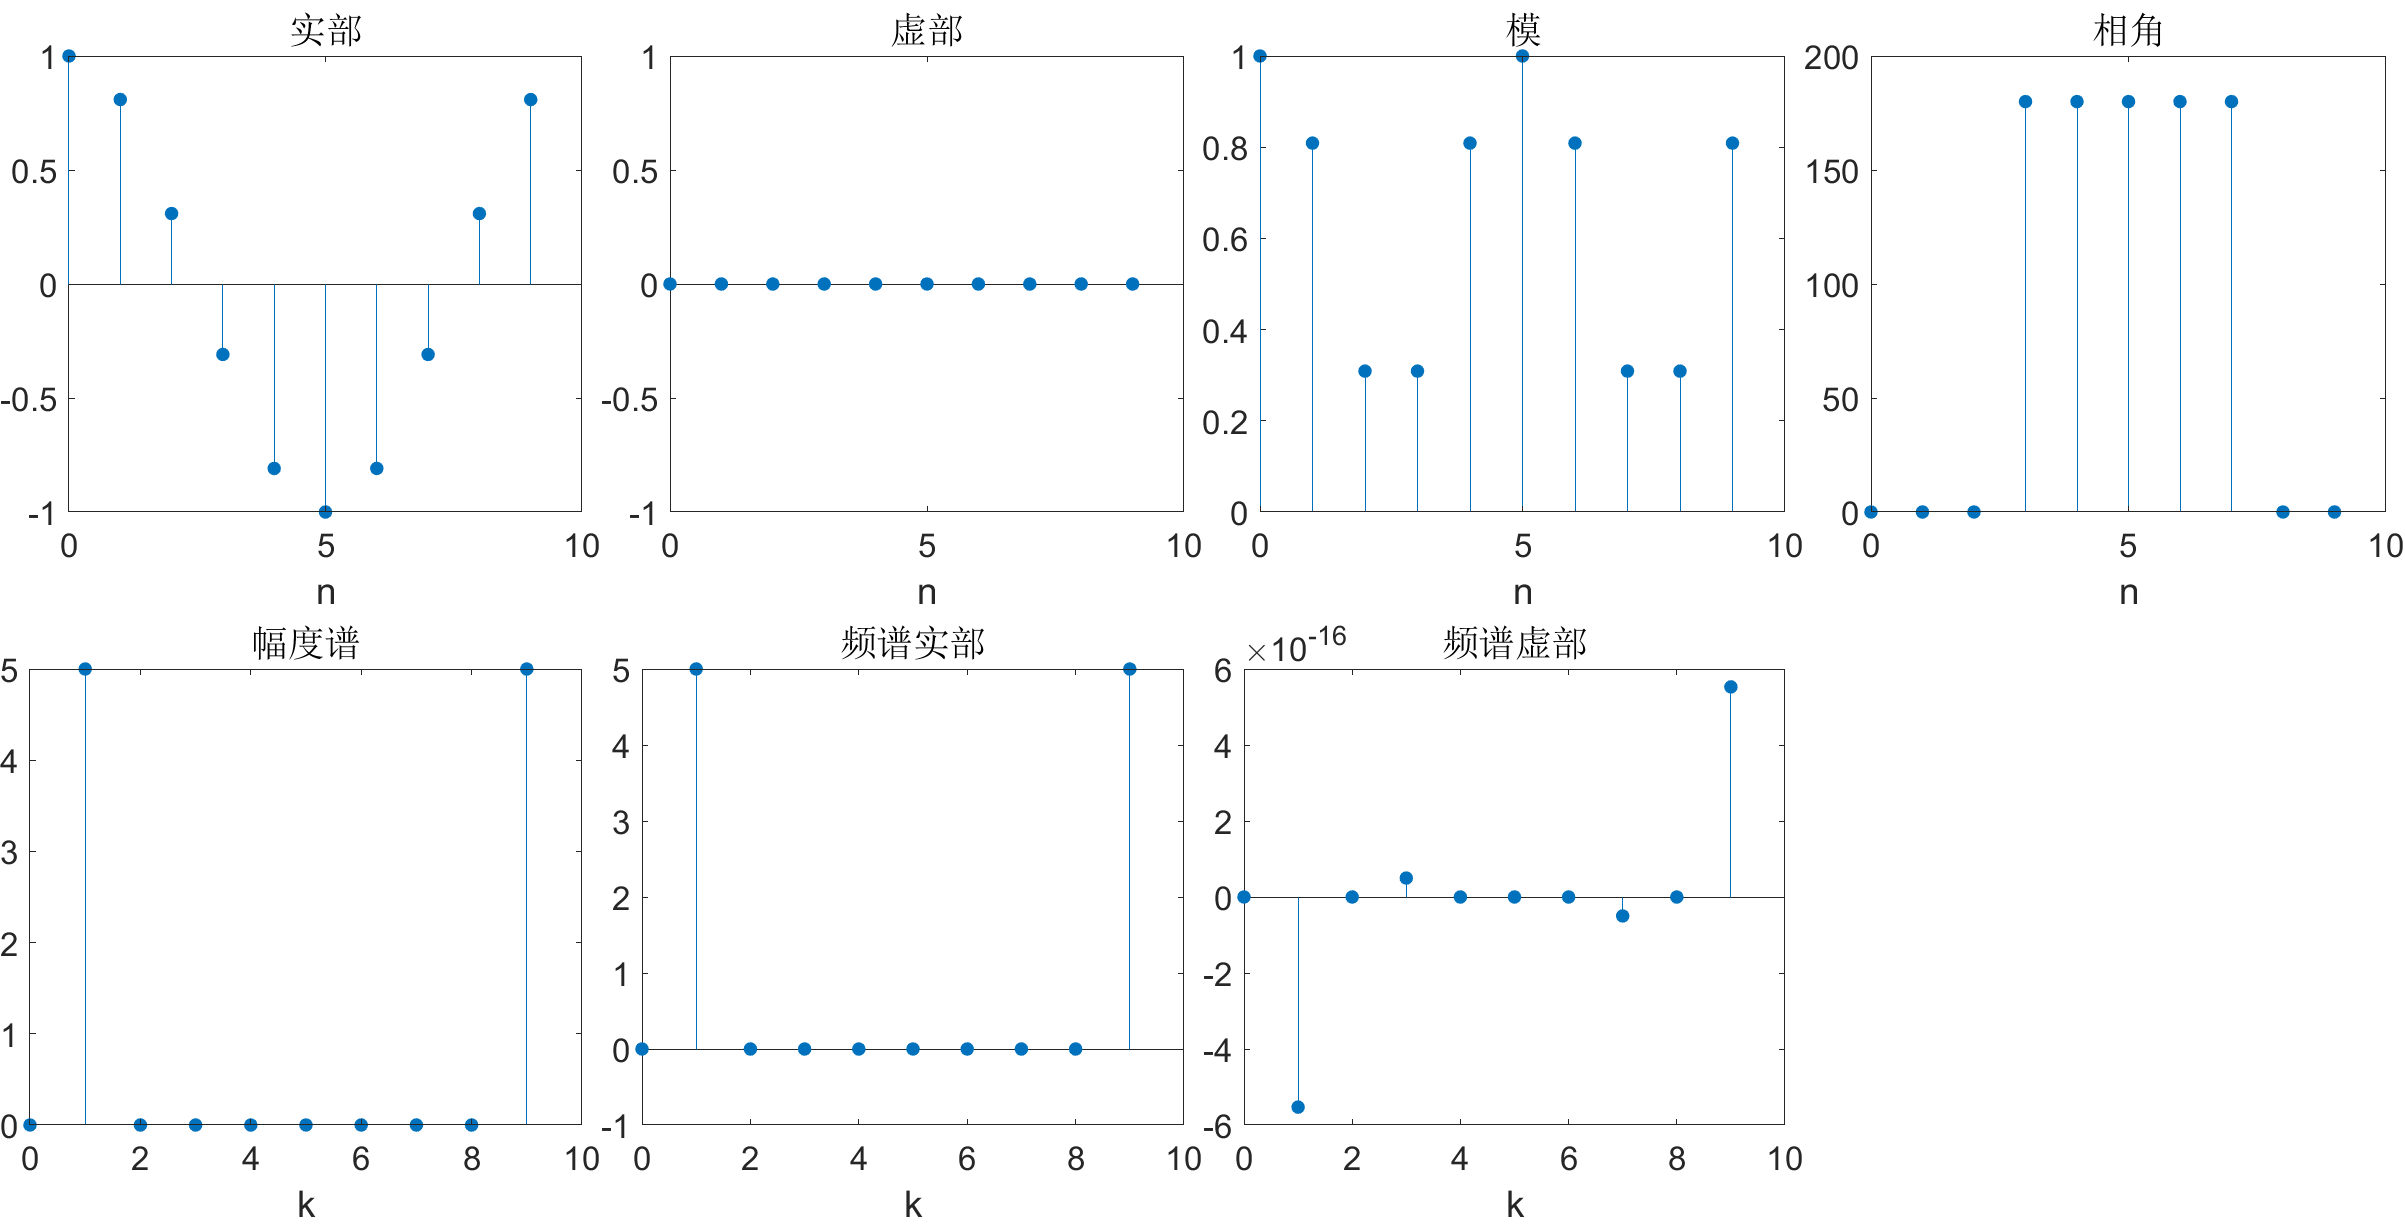
\includegraphics[width = \textwidth]{src/2_1_4.png}
                \caption{余弦函数抽样序列}
            \end{figure}

            由时域图可知,此序列为偶对称序列。模为偶对称,且其相位在x(n)小于零时为0,在大于零时为180\degree
            由频域图可知,因为该序列的对称性,所以频谱的虚部趋于 0。

            \subsubsection{含两个频率分量的复合函数序列$x(n)=sin(2\pi f_1 n T)+delta \times sin(2\pi f_2 nT+phi)$。}

            \begin{figure}[H]
                \centering
                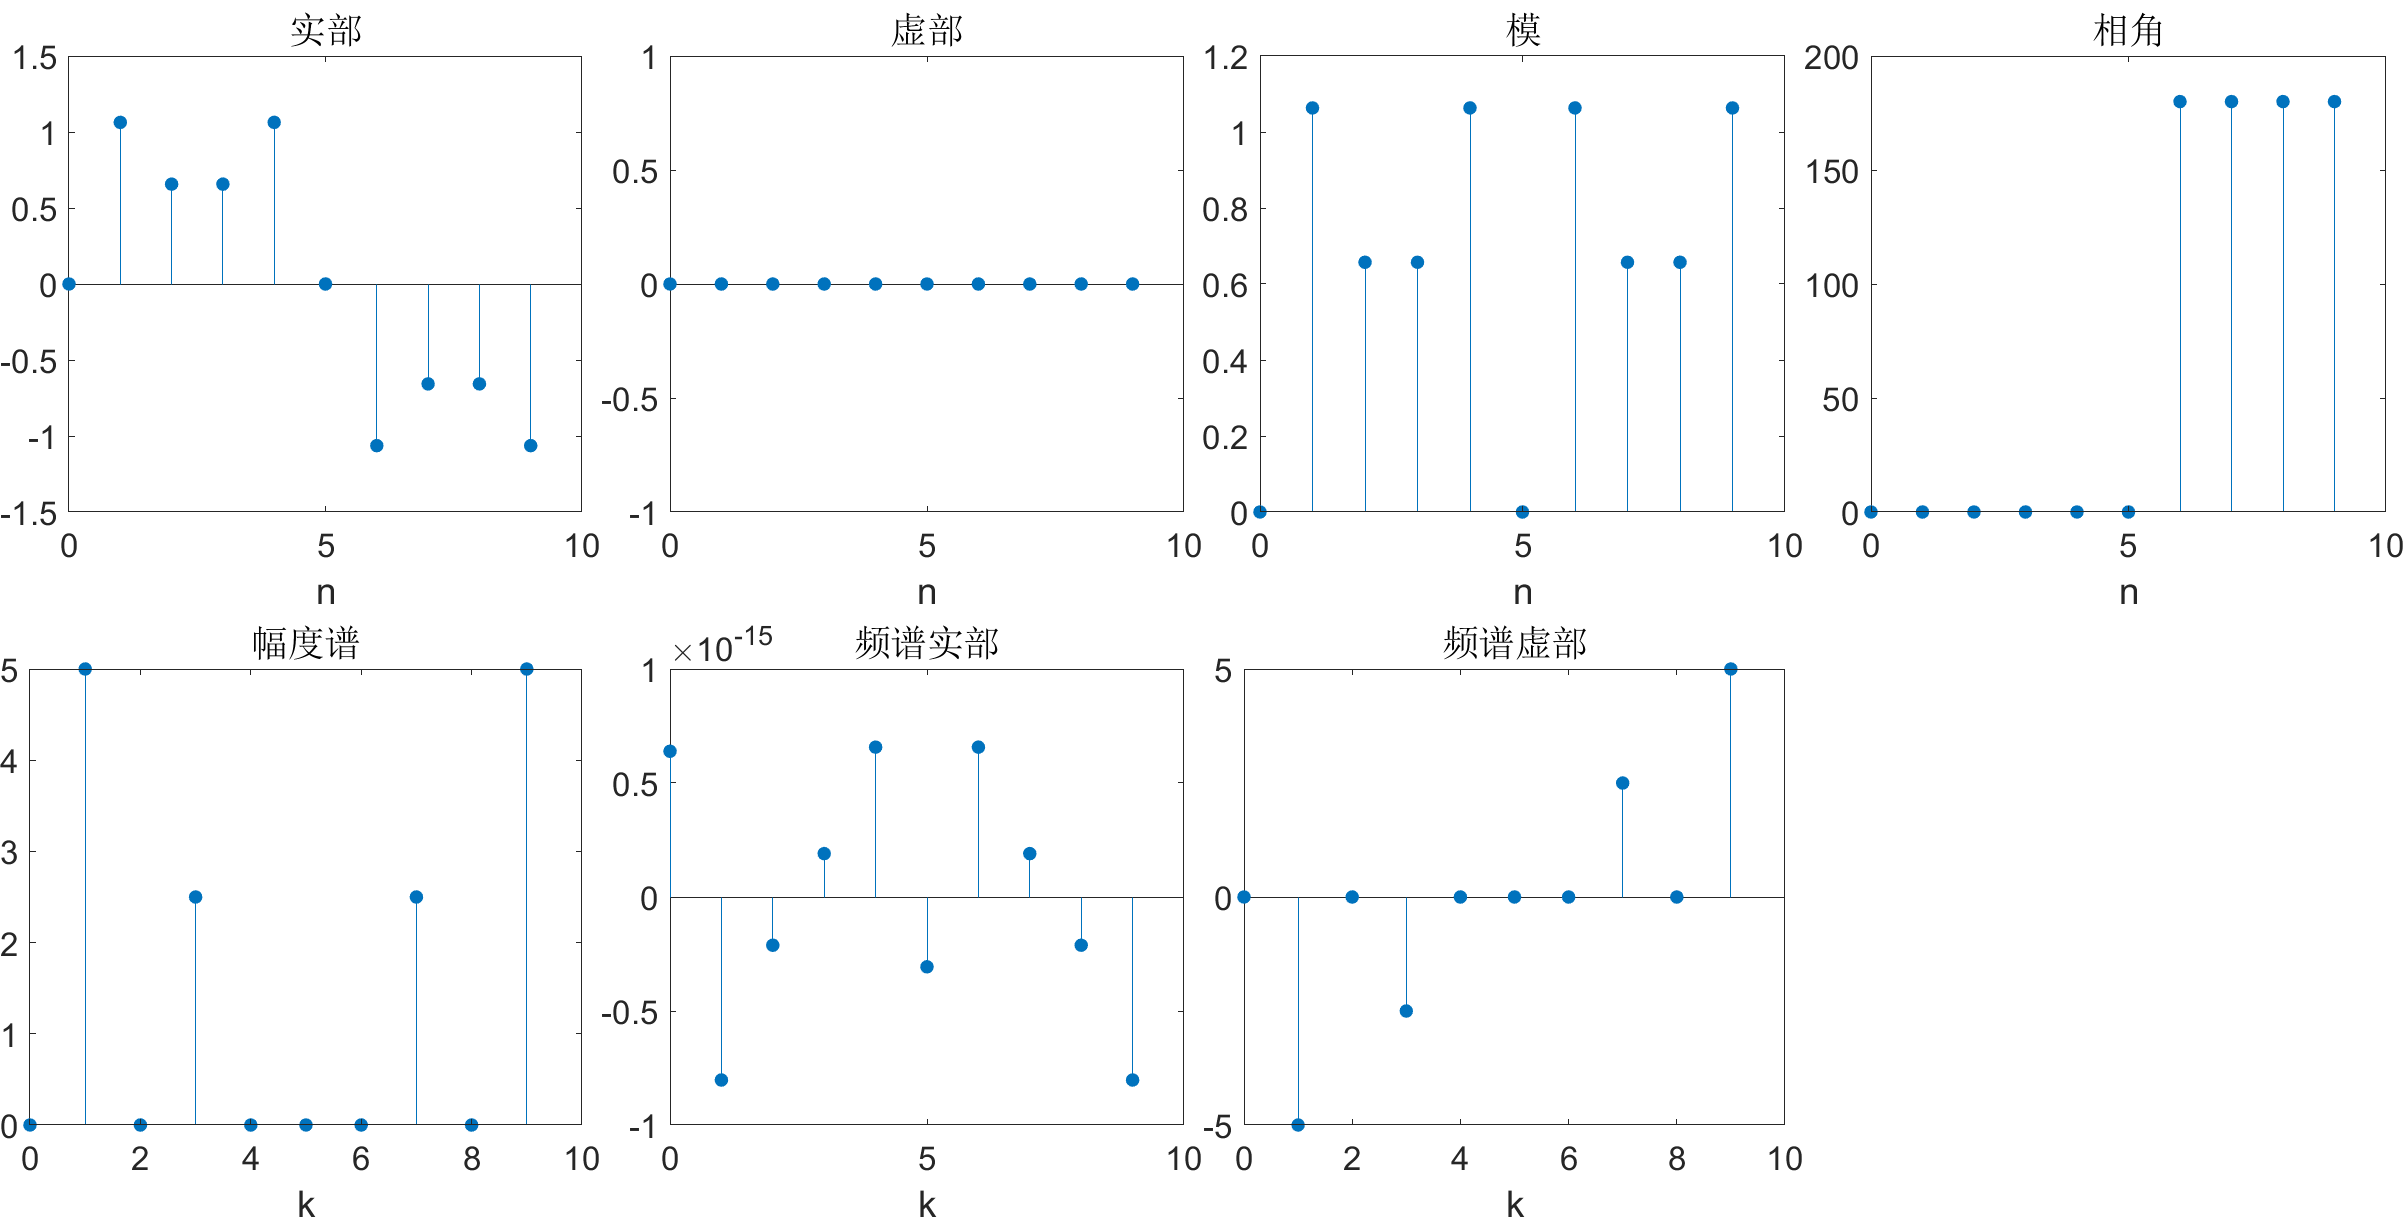
\includegraphics[width = \textwidth]{src/2_1_5a.png}
            \end{figure}
            \begin{figure}[H]
                \centering
                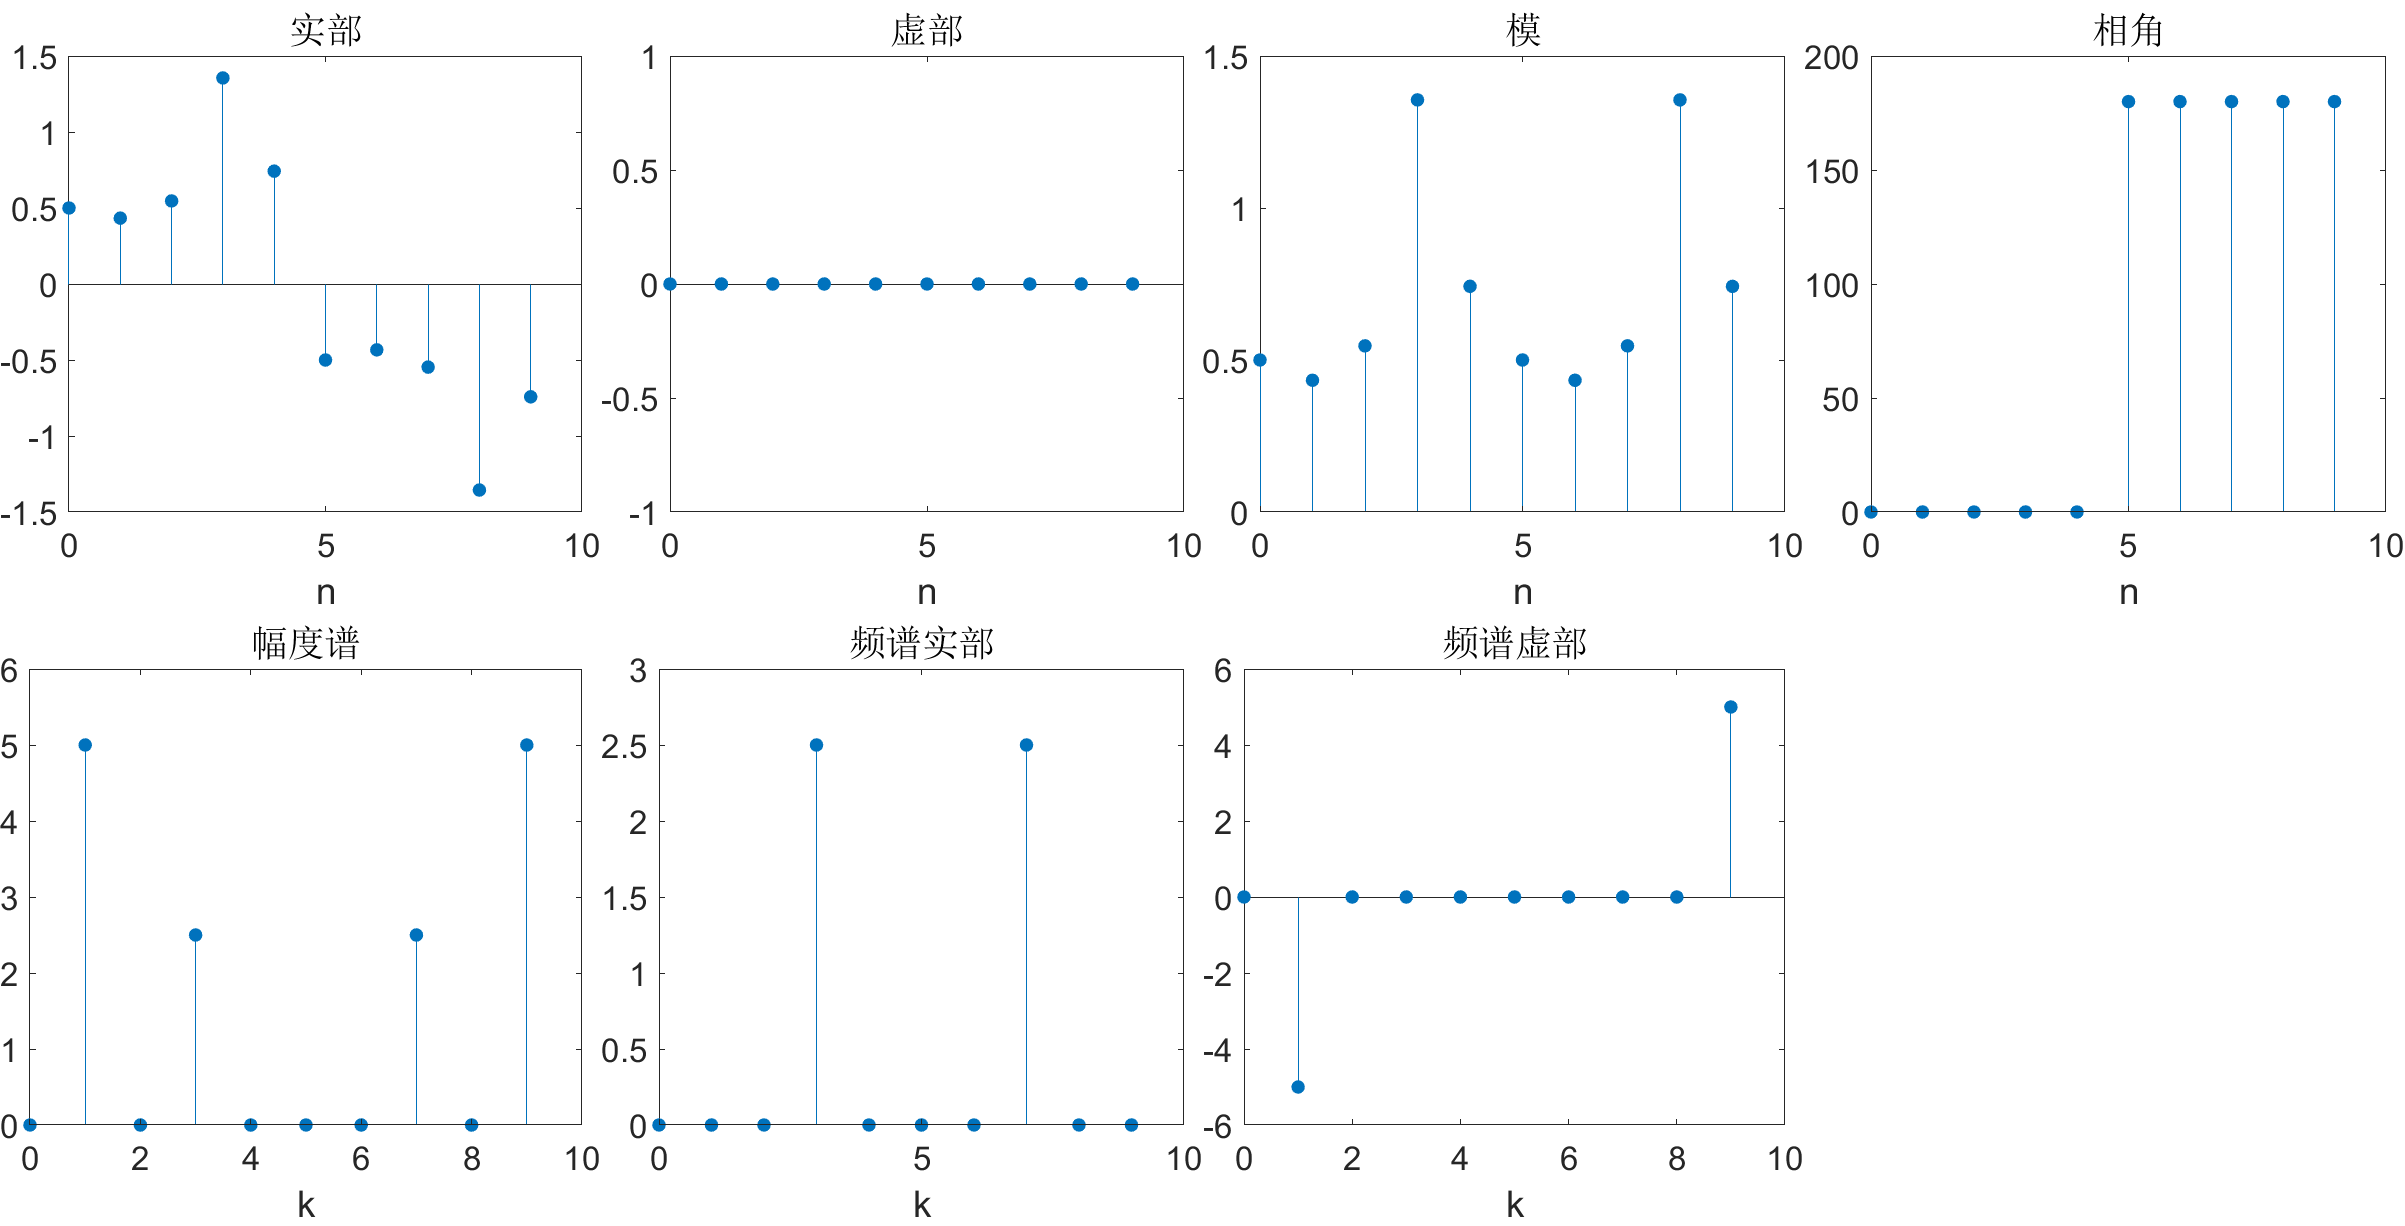
\includegraphics[width = \textwidth]{src/2_1_5b.png}
            \end{figure}
            \begin{figure}[H]
                \centering
                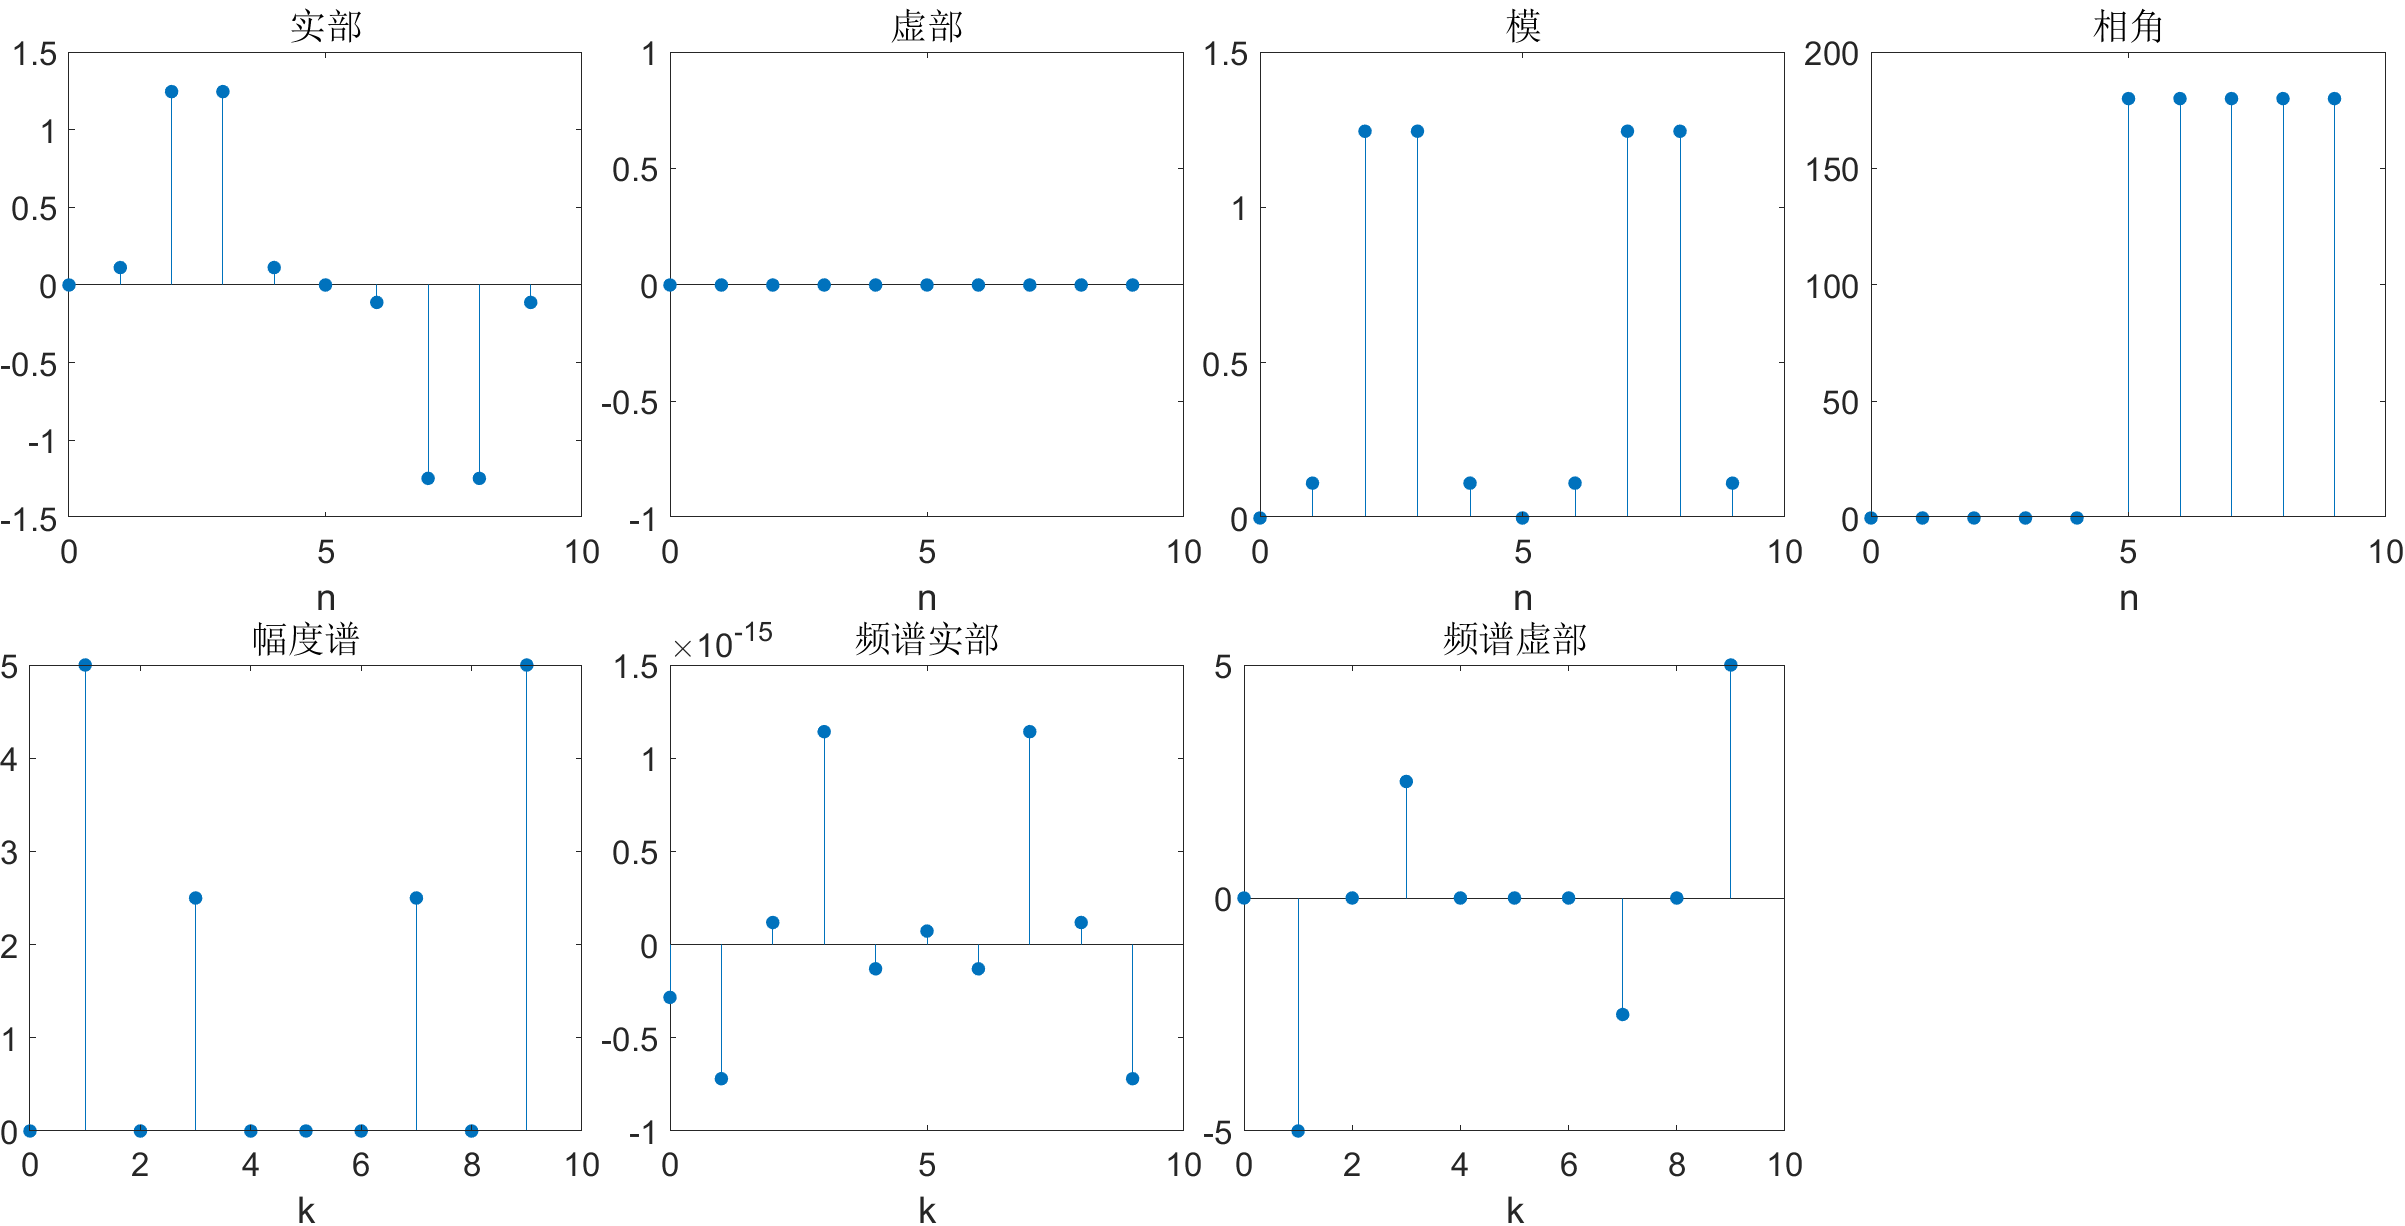
\includegraphics[width = \textwidth]{src/2_1_5c.png}
            \end{figure}

            此序列为是序列,是一个由频率为 1Hz 和频率为 3Hz 的两个序列复合而成。
            当 phi 为 90 时,该序列无对称性。
            当 phi 为 0和 180 时,该序列为奇序列,虚部奇对称。
        \subsection{DFT物理意义。X(0)、X(1)和X(N-1)的物理意义。}
        
        DFT为一个序列傅里叶变换在$0 \sim 2\pi$上的等距离采样。

        X(0):为信号直流分量频谱值。

        X(1):为信号基频处的幅度和相位。

        X(N-1):为信号于N-1次谐波处的幅度和相位。

        \subsection{DFT的主要性质。}
            \subsubsection{线性}
            若$x(n)$和$y(n)$的DFT为$X(k)$与$Y(k)$,则$ax(n)+bx(n)$的DFT为$aX(k)$与$bY(k)$。
            \subsubsection{反转定理}
            若$x(n)$ 的 DFT 结果为 $X(k)$,则 $x((-n))_N$ 的 DFT 为 $X((-k))_N$
            \subsubsection{序列的循环位移}

            若 $x(n)$ 的 DFT 结果为 $X(k)$,$x((n + m))_N$ 的 DFT 为 $W_{N}^{-k m} X(k)$
            \subsubsection{对称性}
            若 $x(n)$ 的 DFT 结果为 $X(k)$,
            
            (1) $x^{*}(n) \underset{\text { IDFT }}{\stackrel{\text { DFT }}{\rightleftharpoons}} X^{*}((-k))_{N}$

            (2) $x^{*}((-n))_{N} \underset{\mathrm{IDFT}}{\stackrel{\mathrm{DFT}}{\rightleftharpoons}} X^{*}(k)$

            (3) $\operatorname{Re}[x(n)] \underset{\mathrm{IDFT}}{\stackrel{\mathrm{DFT}}{\longrightarrow}} X_{\mathrm{e}}(k)$

            (4) $\mathrm{jIm}[x(n)] \underset{\mathrm{IDFT}}{\stackrel{\mathrm{DFT}}{\rightleftharpoons}} X_{\circ}(k)$

            (5) $x_{\mathrm{e}}(n) \underset{\mathrm{IDFT}}{\stackrel{\mathrm{DFT}}{\rightleftharpoons}} \operatorname{Re}[X(k)]$

            (6) $x_{\circ}(n) \underset{\text { IDFT }}{\stackrel{\text { DFT }}{\longrightarrow}} \operatorname{Im}[X(k)]$

            如果 $x(n)$ 为实序列,那么
            (7) $X(k)=X^{*}((-k))_{N}$

            (8) $\operatorname{Re}[X(k)]=\operatorname{Re}\left[X((-k))_{N}\right]$

            (9) $\operatorname{Im}[X(k)]=-\operatorname{Im}\left[X((-k))_{N}\right]$

            (10) $\arg [X(k)]=-\arg \left[X((-k))_{N}\right]$
            \subsubsection{卷积性}
            两个序列圆卷积的DFT为其DFT的乘积。
            \subsubsection{帕斯瓦尔定理}
            $\sum_{n=0}^{N-1}|x(n)|^{2}=\frac{1}{N} \sum_{k=0}^{N-1}|X(k)|^{2}$
 
\end{document}